\documentclass{../src/bcthesispart}
\title{Naming Games}
\author{Bas Cornelissen}
\begin{document}
%——————————————————————————————————————————————————————————
\parttitle{Naming Games}%
	{Naming Games}%
	{naming-games}{%
	% Abstract
	%---------
	How can a population negotiate a shared language without central coordination?
	This is the terrain of naming games, the second class of agent-based models. 
	In local, horizontal interactions, agents 'align' their language until they reach coherence.
	We discuss several alignment strategies, some of which return in later chapters, and conclude with a proof suggesting that a stable, single-word language always emerges.
	The model used therein is the stepping stone for the next chapter, where we connect naming games to Bayesian models of iterated learning.
	}
%——————————————————————————————————————————————————————————


\noindent
\emph{Naming games} (\textsc{ng}) or language games were pioneered in the 90s by Luc Steels and colleagues.
The view of language that motivated their work was similar to the views expressed in the iterated learning literature.
As \textcite{Steels1995} puts it, “language is an autonomous adaptive system, which forms itself in a self-organising process”.
However, language games approach the adaptive system from a different angle than iterated learning.
The development of linguistic structure is not primarily driven by transmission, as Kirby and others proposed, but “by the need to optimise \emph{communicative success}” (p.~319, my italics).
The central question takes the form \parencite{Steels2011}: how can a convention of some sort (lexical, grammatical, or otherwise) emerge in and spread through a population as a result of local communicative interactions, that is, without central coordination?
So if iterated learning is a model of \emph{vertical} language evolution, then the naming games model \emph{horizontal} language evolution.
%%




One of the first studies to explore this, \textcite{Steels1995}, used a game in which (software) agents negotiated a spatial vocabulary.
Equipped with a primitive perceptual apparatus, the agents learned to identify each other by name or spatial position in a shared simulated environment.
Later research extended this approach to embodied robotic agents, grounding their ‘language’ in the physical world.
These \emph{grounded naming games} \parencite{Steels2012,Steels2015} introduce additional complexities pertaining to the perceptual and motor systems of the robots.
We focus on non-grounded games, which can be divided into two branches.
The first is centred around the \emph{minimal naming game}, studied extensively using methods from statistical physics.
The second extended the first naming games to more complex and possibly realistic linguistic scenarios.
This chapter discusses and compares both branches.
Of particular interest is the kind of dynamics one can expect from these models.
We therefore conclude with the proof by \textcite{DeVylder2006} suggesting that naming games always converge to a stable, single-word language.
%%




%——————————————————————————————————————————————————————————
%——————————————————————————————————————————————————————————
\section{The basic naming game}
%——————————————————————————————————————————————————————————
%——————————————————————————————————————————————————————————

Picture a group of people encountering a colourless green object for which they do not have a name. 
Of even worse, suppose they don’t have a shared language at all.
Confused, I suppose, they furiously shout out names for the object.
But can they gradually align their vocabularies by carefully attending to what the others are saying, until they have agreed on a word for the object —
\emph{gavagai}, perhaps?
%%



Frivolities aside, this is the essence of the naming game.
It imagines a population of $N$ agents in a shared environment filled with objects, which the agents try to name.
At the start of the game, there is no agreement whatsoever about the names of the objects.
Every agent has an inventory of names for the objects (a lexicon), which is adjusted after every round with the goal of increasing communicative success.
In every round, two randomly selected agents interact, one as speaker, one as the hearer, according to the following script \parencite{Wellens2012}:
%...
\begin{enumerate}
	\item The speaker selects one of the objects which is to serve as the \emph{topic} of the interaction. She\footnote{%
		% >>>
			‘Gender’ is only introduced to convieniently disambiguate the intended agent: the \emph{s}peaker (she) or the \emph{h}earer (he).
			This even puts the ‘men’ in the role of listener — which I belief is sometimes regarded to be the appropriate role.
		% <<<
		}
		produces a name for the object, either by using one of the names she already knew, or by inventing a new name.
		
	\item The hearer receives the word, interprets it and points to the object he believes was intended.
	
	\item The speaker indicates whether she agrees or disagrees, in that way signalling whether communication was successful.
	
	\item Both the speaker and hearer can update their inventories.
\end{enumerate}
%...




The script is a broad outline and concrete implementations are more specific.
How, for example, does the speaker select a word in step 1?
The typical assumption is that the speaker uses her own experience as a proxy of the hearer’s inventory and opts for a signal she would likely interpret correctly herself.
This is a so called \emph{obverter} strategy \parencite{Oliphant1996}.
Or more importantly, how do the speaker and hearer update their lexicons after the encounter?
Here, the sky is the limit. 
Does the speaker update her lexicon, or the hearer, or both?
What happens after successful communications, what after failure?
In years of research, one particular script emerged, which is discussed below.
It also became clear that whichever update strategy is used, it must improve the \emph{alignment} between the lexicons \textcite{Steels2011}.
That means that the probability that a future encounter will be successful is increased.
Such strategies thus reinforce successfully communicated words and this often installs a winner-takes all dynamics which, in the end, leads to a (unique) shared convention.
This is best seen in the so called \emph{minimal naming game}.
%%




%——————————————————————————————————————————————————————————
%——————————————————————————————————————————————————————————
\section{The minimal strategy}
%——————————————————————————————————————————————————————————
%——————————————————————————————————————————————————————————



The \emph{minimal naming game} was introduced by statistical physicist Andrea Baronchelli (2006)\nocite{Baronchelli2006} and simplifies earlier naming game in several respects \parencite{Baronchelli2006a}.
First, it assumes that homonymy cannot occur.
Homonymy can only be introduced when a speaker invents a \emph{new} word for an object that happens to have been used already to name another object. 
If the space of possible new words is large enough, we can safely assume that invented words are unique and homonymy will be absent.
Secondly, one can assume, without loss of generality, that there is only one object.
If there is no homonymy, the update in step 4 will never affect words used for a different object.
The competition between the synonyms for a particular object is thus completely independent from other objects.
As a result, the dynamics of a naming game with multiple objects is fully determined by the dynamics of a game with a single object.
%%


%- - - - - - - - 
\begin{SCfigure}
	\sffamily\footnotesize\color{main}
	\begin{tabular}{@{}lllll@{}}
		\multicolumn{5}{@{}l@{}}{\color{black}\textbf{A.} Failed communication}\\\toprule
		\textsc{speaker}	& \textsc{hearer} 
			&$\Longrightarrow$ &\textsc{speaker}		& \textsc{hearer}
		\\\cmidrule{1-2}\cmidrule{4-5}
		\textbf{Gavagai}	& Spam 
			&&\textbf{Gavagai}	& Spam\\
		Cofveve				& Foo
			&&Cofveve			& Foo\\
		Spam				&
			&&Spam				&\textbf{Gavagai}\\
		\cmidrule{1-2}\cmidrule{4-5}
	\end{tabular}
	%
	\hfill
	%
	\begin{tabular}{@{}lllll@{}}
		\multicolumn{5}{@{}l@{}}{\color{black}\textbf{B.} Successful communication}\\\toprule
		\textsc{speaker}	& \textsc{hearer} 
			&$\Longrightarrow$ &\textsc{speaker}		& \textsc{hearer}
		\\\cmidrule{1-2}\cmidrule{4-5}
		Gavagai		& \textbf{Spam} 
			&&\textbf{Spam}	& \textbf{Spam}\\
		Cofveve				& Foo &&&\\
		\textbf{Spam}		&&&\\
		\cmidrule{1-2}\cmidrule{4-5}
	\end{tabular}
	
	%---------
	\caption{%
	The updates of the minimal naming game illustrated. 
	If communication fails, the hearer adds the word uttered by the speaker (bold) to its vocabulary. 
	After a success, both empty their vocabularies and keep only the communicated word. 
	%----------
	\figdetails{Figure inspired by \textcite{Wellens2012}.}
	\label{fig:ch3:minimal-naming-game-updates}}
\end{SCfigure}
%- - - - - - - - 




In the minimal naming game, the inventory of every agent is a list of words.
In step 1, the speaker select one word uniformly at random from her inventory.
The update in step 4 distinguishes two cases.
%...
\begin{itemize}
	\item \textbf{Success.} 
	If the hearer knows the word, communication is successful. Both hearer and speaker remove all \emph{other} words from their inventories, yielding two perfectly aligned inventories with one single word.
	
	\item \textbf{Failure.} 
	If the hearer does not know the word, communication fails and the hearer adds the word to his lexicon.
\end{itemize}
%...
Figure \ref{fig:ch3:minimal-naming-game-updates} illustrates how the inventories of agents change after failed and successful communication.
The dynamics of the games can be studied by collecting several statistics \parencite[cf.][]{Baronchelli2017,Wellens2012}, typically with a certain resolution (e.g.\ after every 10 rounds).
Concretely, we measure the following:
%...
\begin{itemize}
	\item \textbf{(Probability of) communicative success $p_s(t)$}.
		The probability that an interaction at time $t$ is successful. These probabilities are estimated by averaging this binary variable over many runs.
		
	\item \textbf{Total word count $N_{\text{total}}(t)$} 
		The total number of words used in the population at time $t$.
		Some authors prefer to divide it by the population size to get the average number of words per agent.
		
	\item \textbf{Unique word count $N_{\text{unique}}(t)$.} 
		The number of unique words used in the population at time $t$.
\end{itemize}
%...
Due to the stochasticity of the games, individual runs vary substantially and can obscure underlying regularities.
Conversely, the behaviour of a single run can suggest regularities that do not generalise.
For that reason, we study the average behaviour of the games, obtained by averaging over many simulation runs.
%%




%——————————————————————————————————————————————————————————
\paragraph{Phenomenology}

The minimal naming game goes through three distinct phases, as illustrated in figure \ref{fig:MNG01-results}. 
In the first phase, most interacting agents will have empty vocabularies and thus invent new words. 
This results in a sharp increase of the number of unique words $N_{\text{unique}}$ in the population.
In the second phase, no new words are invented, but the invented words spread through the population.
Alignment is still low and words will rare rarely be eliminated, so $N_{\text{total}}$ keeps growing.
In the third phase, after the peak of $N_{\text{total}}$, this changes.
Interactions are increasingly likely to be successful, leading to a sharp increase in communicative success and a drop in $N_{\text{total}}$ as more and more words are eliminated.
This also results in the characteristic S-shaped curve of $p_{\text{success}}$.
Eventually the population reaches coherence in the absorbing state where all agents share one unique word and reach perfect communicative success ($N_{\text{unique}} = 1$, $N_{\text{total}} = N$ and $p_{\text{success}} = 1$).




%- - - - - - - - 
\begin{SCfigure}
	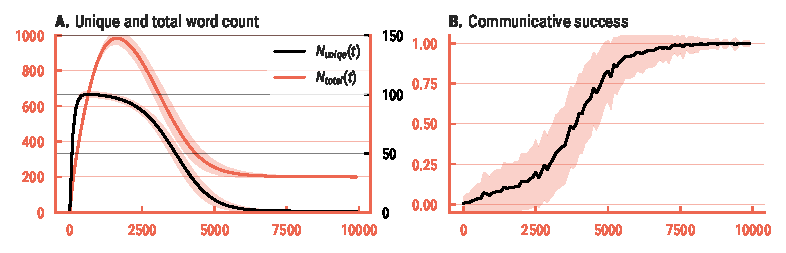
\includegraphics[trim=0.94cm 0 0 \figtopmargin]{MNG01-results}
	
	\caption{
	The dynamics of the minimal naming game.
	An sharp transition leads to convergence and the emergence of consensus.
	%----------
	\figdetails{\figid{MNG01}
	Results shown for $N=200$; avg.\ of 300 runs, 1 std.\ shaded.}
	\label{fig:MNG01-results}}
\end{SCfigure}
%- - - - - - - - 



The game has two important properties, that one might call \emph{effectiveness} and \emph{efficiency}.
The resulting communication system is \emph{effective} because agents learn to communicate successfully, and \emph{efficient} in the sense that agents do not memorise more words than strictly necessary (one, in this case).
A simple argument shows that the minimal naming game almost always reaches an efficient and effective stable state \parencite{Baronchelli2006a}.
At any point in the game, there is a positive probability of reaching coherence in $2(N-1)$ steps: pick one speaker and let her speak to all other $N-1$ agents twice. 
The first time, a hearer might still have to adopt the word, but after the second interaction only one word will remain in his inventory.
If $p$ is the probability of this (unlikely) sequence of interactions, the probability that it has not occurred after $k \cdot 2(N-1)$ steps is less than $(1-p)^k$, which decreases exponentially in $k$.
With probability 1, the population will thus reach coherence as $k \to \infty$.
The argument is somewhat unsatisfactory as it does not reveal anything about the dynamics: how fast is the convergence, for example?
%%




%——————————————————————————————————————————————————————————
\paragraph{Scaling relations and network structure}

To obtain a better insight in the dynamics, one can adopt a methodology commonly used in statistical physics and look at \emph{scaling relations}.
The question is then how certain quantities, like convergence time, \emph{scale} with the size of the system, i.e. the number of agents.
To that end, two critical points are identified: the time $t_{\text{conv}}$ where the game reaches coherence and the time $t_{\text{max}}$ at which point $N_{\text{total}}(t)$ reaches its maximum.
It turns out that these quantities depend on the population size $N$ in a power-law fashion \parencite{Baronchelli2006a,Loreto2011}:
\begin{align}
	\label{eq:ch3:scaling-naming-game}
	t_{\text{conv}}, 
		\; t_{\text{max}},
		\; N_{\text{total}}(t_{\text{max}}) \propto N^\alpha
	 \qquad \text{where $\alpha \approx 1.5$}	
\end{align}
Now note that $N_{\text{total}}(t_{\text{max}}) / N$ is the maximum number of words each agent has to store on average — the maximum memory load, perhaps.
\textcite{Baronchelli2017} concludes that “the cognitive effort an agent has to take, in terms of maximum inventory size, \emph{depends on the system size} and, in particular, diverges as the population gets larger” \parencite[][italics in original]{Baronchelli2017}.
Although interesting, I would be hesitant to concede that linguistic activity in a small language community requires less cognitive effort than the same activity in a larger community.




Besides the scaling effects, the role of the network structure of the population has been studied extensively \parencite[see][for an overview]{Baronchelli2017}.
In the classical naming game any two agents can interact — there is  \emph{homogeneous mixing} — corresponding to a fully connected social network.
Varying the topology (to e.g.~more realistic small-world networks, \cite{DallAsta2006}) strongly influences the dynamics.
This is reflected by different scaling relations, but not by convergence per se: the population still negotiates a unique word — as long as the networks remains connected, of course.




%——————————————————————————————————————————————————————————
\section{Lateral inhibition strategies}

The minimal strategy is somewhat opportunistic in that it forgets all other words after a successful encounter.
It has been suggested that subtler alignment mechanisms might yield faster convergence times: so called \emph{lateral inhibition strategies} (see \cite{Wellens2012} ch.~2, for an overview).
The name is ultimately derived from biology, where excited neurons can be found to \emph{inhibit} neighbouring neurons.
Similarly, lateral inhibition strategies decrease the chance of using competing words again.
To that end, they assign a \emph{score} to every word.
If a word is communicated successfully, its score is increased, and the scores of competitors are decreased or \emph{inhibited}.
The production mechanism must also accounts for the scores, typically by producing the highest-scoring word.




The (basic) lateral inhibition strategy was first formulated in \textcite{Steels2005} and is described by five nonnegative parameters \parencite{Wellens2012}\footnote{%
	%>>>
	\textcite{Wellens2012} only uses $\delta$’s in $(0,1)$, but this general formulation allows the inclusion of the frequency strategy.
	%<<<
	}
%-
\begin{equation}
	\delta_{\text{inc}}, \quad
	\delta_{\text{inh}}, \quad
	\delta_{\text{dec}}, \quad
	s_{\text{init}}, \quad 
	s_{\text{max}}.	
\end{equation}
%-
After a success, both agents increase the score of the communicated word by $\delta_{\text{inc}}$ and decrease scores of competitors by $\delta_{\text{inh}}$. 
After a failure, the hearer adopts the word with score $s_{\text{init}}$ and the speaker decreases the score by $\delta_{\text{dec}}$.
Whenever a score drops below (or equals) 0 the word is removed, and scores can never grow larger than $s_{\text{max}}$.
Other inhibition strategies have also been used and will be discussed in chapter \ref{ch:conclusions}.




The minimal strategy is a special case of the lateral inhibition strategy, for $\delta_{\text{inc}} = \delta_{\text{dec}} = 0$ and $\delta_{\text{inh}} = s_{\text{init}} = 1$ (see also table \ref{table:li-strategies}).
With those parameters new words get score 1 and this score is never further increased. 
It \emph{can} be inhibited, by 1, which leads to to immediate removal.
In this strategy, the scores thus play a purely administrative role.
A strategy where scores play a larger role, is the \emph{frequency strategy} which counts how often every word has been encountered.
This strategy however exhibits no form of lateral inhibition.
The minimal strategy and frequency strategy thus mark two extremes: the former has the strongest possible form of lateral inhibition, the latter none.
Between these endpoints lie the proper lateral inhibition strategies.




%- - - - - - - -
\begin{SCtable}\sffamily\footnotesize\color{main}
	\begin{tabular}{@{}lllllll@{}}
		\toprule
		& $\delta_{\text{inc}}$ 
		&$\delta_{\text{inh}}$ 
		&$\delta_{\text{dec}}$ 
		&$s_{\text{init}}$ 
		&$s_{\text{max}}$\\\midrule
		\textsc{minimal strategy}		&0	&1	&0	&1 	&$1$\\
		\textsc{lat.~inhibition strategy 1}		&1	&1	&0	&1 	&$\infty$\\
		\textsc{lat.~inhibition strategy 2}		&0.1	 &0.5	&0.1	&0.5	&$1$\\
		\textsc{lat.~inhibition strategy 3}		&0.1	 &0.2	&0.2&0.5	&$1$\\
		\textsc{frequency strategy}		&1	&0	&0	&1	&$\infty$\\
		\bottomrule	
	\end{tabular}
	\caption{Parameter settings for four different strategies, whose behaviour is shown in figure \ref{fig:LING01-strategies}. Note that equivalent parametrisations also exist; see main text for details.
		\label{table:li-strategies}}
\end{SCtable}
%- - - - - - - -


%- - - - - - - -
\begin{SCfigure}
	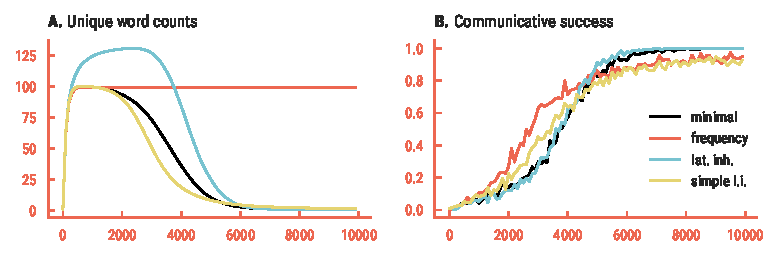
\includegraphics[trim=0.8cm 0 0 \figtopmargin]{LING01-results}
	
	\caption{
	Comparison of the four naming game strategies in table \ref{table:li-strategies}. 
	The the unique word count and communicative success show that all strategies reach communicative success. 
	The stable language for the frequency strategy is not efficient.
	%----------
	\figdetails{\figid{LING01}
	Results shown for $N=200$; avg.\ of 300 runs. $p_{\text{success}}$ is a rolling average over a centered window of 1000 iterations.}
	\label{fig:LING01-strategies}}
\end{SCfigure}
%- - - - - - - -




I want to discuss three fairly different \textsc{li} strategies here: 
\textsc{li} strategy 1 is a strategy that returns in chapter \ref{ch:counting-games}; 
strategy 2 is taken from \textcite{Wellens2012}; 
and strategy 3 is a variation thereof.
The parameters are listed in table \ref{table:li-strategies} and figure \ref{fig:LING01-strategies} shows the dynamics.
First of all note that the dynamics of $N_{\text{unique}}$ can strongly differ for different strategies (subfigure \textsc{a}).
If for example $\delta_{\text{inh}} = \delta_{\text{dec}}$ as in \textsc{li} strategy 3, many more words can be invented.
But eventually this strategy gives rise to an efficient language.
So do all other strategies, except that the frequency strategy results in a maximally inefficient languages where all agents know all words.
Since agents only use the most frequent word, perfect communicative accuracy is still attained, as is the case for the other strategies.
%%




These are just five strategies, but what does the rest of the strategy space look like?
In appendix \ref{app:li-strategies} I systematically explore a larger part of the space, following \textcite{Wellens2012}.
I indeed find that $\delta_{\text{inh}}$ interpolates between the minimal and frequency strategy.
Further, relatively large $\delta_{\text{inc}}$ can lead to temporary stabilisation at a non-equilibrium state, until inhibition takes over the stable state is reached.
However, I should note that I do not replicate Wellens’s finding that the frequency converges faster than the minimal strategy (see also figure \ref{fig:LING01-strategies}), and have not been able to reconstruct why.
Although the behaviour might vary initially, the long-term behaviour is unaffected: convergence to a single-word language.
%%




In sum, all strategies discussed allow the population to solves the naming problem and leads to effective communication within the population.
Any form of lateral inhibition dampens competing words, a result of which agents eventually forget all but one word.
The frequency strategy is the only discussed strategy that is not \emph{efficient} in this sense.
For different parameter settings communicative success can increase earlier, later or even stabilise temporarily, but will eventually be reached nonetheless.
Indeed, it seems that “adding a scoring mechanism yields only marginal improvements in terms of communicative and alignment success” \parencite[23]{Wellens2012}\footnote{%
	%>>>
	That is, for the basic naming game, since \textcite{Wellens2012} finds that in more complicated games, subtle update mechanisms \emph{can} be beneficial.
	%<<<
	}
Why, one wonders, is the convergence so robust? 
%%




%——————————————————————————————————————————————————————————
%——————————————————————————————————————————————————————————
\section{Proof of convergence}
%——————————————————————————————————————————————————————————
%——————————————————————————————————————————————————————————

To the best of my knowledge, \textcite{DeVylder2006} provided the only analytical result indicating that non-minimal naming games converge to a shared, single-word language.
The results apply to a variant of the game, which makes similar simplifications as the minimal naming game: there is no homonymy and only a single object.
It moreover starts ‘later’ in the game, when all agents have already engaged in an interaction and no new words are invented.
At this point, there are $K$ unique words $w_1, \dots w_K$ in the game and the authors assume none of these is ever removed — very much like the frequency strategy.
Similarly, speakers use observed frequencies to determine which word they will produce.
For production strategies that reinforce or amplify the most frequent word, the authors are able to prove convergence to a single-word language.
However, their proof applies to a \emph{deterministic} model, the \emph{sampling-response model}, and De Vylder and Tuyls use simulations — not a proof — to argue that their results generalise to the actual \emph{stochastic}, \emph{turn-based model}.
I will present the deterministic, \emph{sampling-response} model in some detail, partly because it is the stepping stone for the next chapter.
%%




%- - - - - - - 
\begin{SCfigure}
	%\documentclass{../src/bcthesispart}
%\begin{document}
\tdplotsetmaincoords{70}{60}
	\begin{tikzpicture}[scale=3,tdplot_main_coords]\footnotesize
		\def\laxis{1.2}
		\def\ltriangle{1}
		\def\ltick{.1}
		%%% axes
		\draw [->,main] (0,0,0) -- (\laxis,0,0) node [below] {$\lang_1$};
		\draw [->,main] (0,0,0) -- (0,\laxis,0) node [right] {$\lang_2$};
		\draw [->,main] (0,0,0) -- (0,0,\laxis) node [left] {$\lang_3$};
		%%% axes ticks
		\begin{scope}[
		help lines,
		every node/.style={inner sep=1pt,text=black}
		]
		\foreach \coord in {1} {%{1,...,\nticks} {
		  \draw [main] (\coord,\ltick,0) -- ++(0,-\ltick,0) -- ++(0,0,\ltick)
		  node [at start,below left,main] {\coord};
		  \draw [main] (\ltick,\coord,0) -- ++(-\ltick,0,0) -- ++(0,0,\ltick)
		  node [pos=1,right,main] {\coord};
		  \draw [main] (\ltick,0,\coord) -- ++(-\ltick,0,0) -- ++(0,\ltick,0)
		  node [at start,above left,main] {\coord};
		}
		\end{scope}
		%% Example vector
		\draw [dashed,main] (.2,0,.8) -- (.2,.8,0);
		\draw [dashed,main] (0,.3,.7) -- (.7,.3,0);
		\draw[->,line width=.5](0,0,0) -- (0.2,0.3,0.5) node[at end,above right] {$\vlang = (0.2,0.3,0.5)$};
		%%% figure
		\filldraw [opacity=.3,main] (\ltriangle,0,0) -- (0,\ltriangle,0)
		-- (0,0,\ltriangle) -- cycle;
	\end{tikzpicture}
	%
	\begin{tikzpicture}[scale=3]\footnotesize
	
	    % draw the background
	    \draw [fill=main!30] (0,0) -- (60:1) -- (1,0) -- cycle;
	
	    \coordinate[label=left:{\color{main}$(1,0,0)$}]  (A) at (0,0);
	    \coordinate[label=right:{\color{main}$(0,1,0)$},main] (B) at (1,0);
	    \coordinate[label=above:{\color{main}$(0,0,1)$},main] (C) at (60:1);
	
	    % the triangle
	    \draw [line width=.5pt,main] (A) -- (B) -- (C) -- cycle;
	    
	    % y = sqrt(3) / 2 * (1-theta_2)
	    % x = 1/2*theta_2 + 1/2
	    \draw [dashed,main] (.3,0) -- (0.65,0.60621) 
	    	node [main,at end, above right] {$\lang_2 =0.3$};
	    \draw [dashed,main] (.8,0) -- (60:.8)
	    	node [main,at end, above left] {$\lang_1 = 0.2$};
		
		% x = sqrt(3) / 2 * theta_3
		% y = theta_2 + 1/2 * theta_3
	    \draw [fill=black] (.55, 0.4330) circle[radius=.5pt];
	    
	    \draw [decoration={brace,mirror,raise=0.1cm}, decorate] (0,0) -- (.3,0)
	   		node [pos=0.5,yshift=-0.5cm] {$\lang_2$}; 
	    \draw [decoration={brace,mirror,raise=0.1cm}, decorate] (.3,0) -- (.8,0)
	   		node [pos=0.5,yshift=-0.5cm] {$\lang_3$}; 
	    \draw [decoration={brace,mirror,raise=0.1cm}, decorate] (.8,0) -- (1,0)
	   		node [pos=0.5,yshift=-0.5cm] {$\lang_1$}; 
	   		
		\begin{scope}[xshift=1.6cm]
			\def\barwidth{.12}
			\def\gap{.03}
			\def\tick{.02}
			
			\tikzset{bar/.style={draw=main,fill=main!30}}
			\draw[bar] (0,0) rectangle (\barwidth,.2);
			\draw[bar] (\barwidth+\gap,0) rectangle (2*\barwidth+\gap,.3);
			\draw[bar] (2*\barwidth+2*\gap, 0) rectangle (3*\barwidth+2*\gap, .5);
			
			% Axis
			\draw (-\gap,0) -- (3*\barwidth+3*\gap,0);
			\draw (.5*\barwidth, -\tick) -- (.5*\barwidth, \tick);
			\node at (.5*\barwidth, -4*\tick) {$\lang_1$};
			
			\draw (1.5*\barwidth+\gap, -\tick) -- (1.5*\barwidth+\gap, \tick);
			\node at ((1.5*\barwidth+\gap, -4*\tick) {$\lang_2$};
			
			\draw (2.5*\barwidth+2*\gap, -\tick) -- (2.5*\barwidth+2*\gap, \tick);
			\node at (2.5*\barwidth+2*\gap, -4*\tick) {$\lang_3$};
		\end{scope}
	\end{tikzpicture}
%\end{document}

	
	\caption{%
	A discrete distribution $\vlang$ over three values corresponds to a point in the $2$-simplex, a triangular slice of $\mathbb{R}^3$ (left).
	The simplex can be embedded in the plane (middle), so that every point in the triangle determines a distribution (right).
	\label{fig:ch3:simplex}
  }
\end{SCfigure}
%- - - - - - - 




%——————————————————————————————————————————————————————————
\paragraph{Preliminaries}

First of all, we need to introduce the \emph{simplex}: the space of discrete probability distributions.
A probability distribution over $K$ words is described by a vector $\vlang = (\lang_1, \dots, \lang_K)$ such that all $\lang_k$ are positive, and they together sum to 1, i.e.\ $\sum_k \lang_k = 1$.
Note that the last entry, $\lang_K$, is determined by the others and constraint $\sum_k \lang_k = 1$.
Probability vectors therefore lie in a $(K-1)$-dimensional slice of $\mathbb{R}^K$.
This slice is known as the $(K-1)$-\emph{simplex} $\simplex^{K-1}$, or simply $\simplex$ if no confusion can arise.
The 2-simplex corresponds to a triangle, as illustrated in figure \ref{fig:ch3:simplex}.
%%



The model proposed by \textcite{DeVylder2006} considers a population of $N$ agents who keep a queue of the last $Q$ words they have observed.\footnote{%
	%>>>
		The notation of \textcite{DeVylder2006} maps to ours as follows: 
			${n \rightsquigarrow K}$,
			${K \rightsquigarrow Q}$,
			${m_i \rightsquigarrow c_i}$,
			${x_i \rightsquigarrow q_i}$,
			${s(k) \rightsquigarrow \pi_k}$
			${\Sigma \rightsquigarrow \Delta}$,
			${\sigma \rightsquigarrow \vect\theta}$ (mostly), and
			${\tau \rightsquigarrow \bar{\vect\pi}}$.
		% <<<
	} 
A speaker will utter a word based on the relative frequencies of the words in her queue. 
Formally, we write $\vect c=(c_1, \dots, c_K)$ for the vector of \emph{counts}, i.e. $c_k$ the the number of $k$’s in the queue.
The counts correspond to (relative) frequencies $\vlang = (\lang_1, \dots, \lang_K)$ where $\lang_k = c_k / Q$.
The point $\vlang = (0.2, 0.3, 0.5)$ in figure \ref{fig:ch3:simplex} for example depicts the frequencies of $K=3$ words in a queue of length $Q=10$ with 2 occurrences of $w_1$, 3 of $w_2$ and 5 of $w_3$.
By ‘frequencies’ $\vlang$ we from now on mean \emph{relative} frequencies and we also call $\vlang$ the \emph{language} of an agent.
The frequencies lie in a discrete subset $\simplex_Q$ of the simplex which depends on the size of the queue $Q$ (see figure \ref{fig:discrete-simplex}).




%- - - - - - -
\begin{SCfigure}	
	%\documentclass{../src/bcthesispart}
%\begin{document}

\begin{tikzpicture}[scale=5.2]\footnotesize\sffamily
	\tikzset{point/.style={fill=black}}
	\newcommand{\discretesimplex}[1]{
    	% draw the triangle
	    \fill [color=main!30] (0,0) -- (60:1) -- (1,0) -- cycle;
	    \coordinate (A) at (0,0);
	    \coordinate (B) at (1,0);
	    \coordinate (C) at (60:1);
	    \draw [line width=.5pt,main!50] (A) -- (B) -- (C) -- cycle;
    	
    	% Draw the points
	    \def\Q{#1}
	    \foreach \a in {0,...,\Q} {
	    	\pgfmathsetmacro {\bmax} {int(\Q-\a)}
	    	\foreach \b in {0,...,\bmax} {
		    	\pgfmathsetmacro {\c} {int(\Q-\a-\b)}
			    \draw[point] (barycentric cs:A=\a,B=\b,C=\c) 
			    	circle[radius=.008] node[above=0.05] {\a\b\c};
	    	}
	    }
	    
	    % Label
	    \node at (.5,-.12) {Queue of length \Q};
	}
	
	% Left simplex
	\discretesimplex{4}
	
	% Right simplex
	\begin{scope}[xshift=1.2cm]
		\discretesimplex{6}		
	\end{scope}
\end{tikzpicture}
	
%\end{document}

	
	\caption{
	All possible frequencies of 3 words in a queue of length 4 (left) and 6 (right) form a discrete subset of the simplex. 
	The corresponding relative frequencies are the ‘languages’ used by agents in the sampling-response model.
	Frequencies $(a,b,c)$ are labeled $abc$.
	%----------
	\figdetails{Figure inspired by \parencite{DeVylder2006}.	}
	\label{fig:discrete-simplex}}
\end{SCfigure}
%- - - - - - -



Given a language, a \emph{response function} $r$ determines with what probability each word is uttered.
Consider for example the response function $r$ that puts all mass on the most frequent word.
In our example with $\vlang = (0.2, 0.3, 0.5)$ this means that $r(\vlang) = (0,0,1)$, so the probability of uttering $w_3$ is $p(\obs=w_3 \mid \vlang) = 1$.
More generally, $r: \Delta \to \Delta$ maps the language $\vlang_A$ of agent $A$ to a \emph{word distribution} $\vect\pi_A := r(\vect z_A)$, such that the probability of uttering word $\obs=w_k$ is
%-
\begin{align}
	p(\obs = w_k \mid A) 
		= \pi_{A,k}, 
	\qquad \text{where $\pi_{A,k} = \bigl[r(\vlang_A)\bigr]_k$}
\end{align}
%-
%%




%——————————————————————————————————————————————————————————
\paragraph{the sampling-response model}

It is not easy to analyse this game directly.
Consider how the language $\vlang$ of a hearer changes during an interaction.
The only thing that matters is the probability of hearing a word, not which speaker uttered it.
We obtain those probabilities by averaging over all possible speakers (for simplicity, agents are allowed to speak to themselves),
%-
\begin{align}
	p(x = w_k) 
		= \bar\pi_k, 
	\qquad \text{where} \; 
	\bar{\vecpi} 
		= \frac{1}{N} \sum_{A=1}^N \vect\pi_A,
\end{align}
%-
and call this average word distribution the \emph{aggregate languages} as it aggregates the languages of all agents.
Since the language of the hearer changes in every round, the aggregate language $\bar\vecpi$ also varies from round to round. 
To obtain a analysable model, \textcite{DeVylder2006} nonetheless assume it temporarily remains constant.
In the resulting \emph{sampling-response} model all agents interact synchronously in successive \emph{episodes}.
During an episode all agents simultaneously receive $Q$ utterances, drawn from the aggregate language $\bar{\vect\pi}$.
One episode therefore corresponds to multiple rounds of the original turn-based game, enough to ensure that all agents have ‘flushed’ their queues, i.e.\ acted as a hearer $Q$ times.
Indeed, the analogy is not perfect, but deliberately so.
%%




Importantly, \emph{the sampling-response model is deterministic} and analysing how an agent’s language changes during an episode becomes much easier.
Concretely, if $\bar{\vect\pi}$ is the aggregate language during an episode $t$, the probability of observing frequencies $\vlang_t$ is the probability of observing the corresponding counts $\vect c_t$ amongst $Q$ independent draws from $\bar{\vect\pi}_t$.
A multinomial probability, that is, so the sampling-response model takes the form
%-
\begin{align}
	\vlang_t \mid \bar{\vect\pi}_t
		& \sim \text{Multinomial} \bigl(\vect c_t \mid \bar{\vect\pi}_t \bigr),
		\qquad \vect c_t = Q\cdot \vlang_t, 
	\\
	x_t \mid \vlang_t
		& \sim \text{Categorical}( r(\vlang_t) )
\end{align}
%-
We can use this to compute the word distribution of agent $A$ \emph{after} episode $t$:
%-
\begin{align}
	\pi_{A,k}^{(t+1)}
		&= p(x_{t+1} 
		= w_k \mid A, \bar{\vect\pi}_t)
		\\
		&= \sum_{\vlang \in \Delta_Q} p(x_{t+1} = w_k \mid \vlang) \cdot p(\vlang \mid \bar{\vect\pi}_t) 
		\\
		&= \sum_{\vlang \in \Delta_Q} 
			[r(\vlang)]_k 
			\cdot 
			\text{Multinomial}( \vect c \mid \bar{\vect\pi}_t).
\end{align}
%-
Note that the word distribution does not depend on $A$.
This implies that the next aggregate language is also
%-
\begin{equation}
	\label{eq:ch3:sampling-response-transition}
	%-----
	\bar{\vect \pi}_{t+1} 
		= \sum_{\vlang \in \Delta_Q}	 \vect r(\vlang) \cdot \text{Multinomial}( \vect c \mid \bar{\vect\pi}_t).
\end{equation}
%-
This defines a deterministic transition $\bar{\vect\pi}_t \mapsto \bar{\vect\pi}_{t+1}$ from the aggregate language in one episode to the next.
%%




%——————————————————————————————————————————————————————————
\paragraph{Convergence}

In summary, in episode $t$ of the sampling-response model, all agents simultaneously hear $Q$ words drawn from the aggregate language $\bar{\vect\pi}_t$.
At the end of the episode, all agents have updated their language, resulting in a new aggregate language $\bar{\vect\pi}_{t+1}$.
The new language is a deterministic function of $\bar{\vect\pi}_t$, but also depends on the response function $r$.
\textcite{DeVylder2006} showed that under certain conditions $\bar{\vect\pi}_t$ converges to an aggregate language with only a single word:
%-
\begin{equation}
	\lim_{t\to \infty} \bar{\vect\pi}_t 
		= (0,\dots,0,1,0,\dots, 0).
\end{equation}
%-
Perhaps the most important condition was that the response function must be \emph{amplifying}.
That means, roughly, that the response function increases the probability of producing the most frequent word (with respect to its frequency).
We have already seen the prime example of an amplifying function: the function that \emph{exponentiates} a distribution (see figure \ref{fig:FIG03}):
%-
\begin{align}
	r_\eta(\vlang) 
		= \frac{1}{\sum_{k=1}^K \lang_k^\zeta} 
			\cdot \Bigl(\lang_1^\zeta, \dots, \lang_K^\zeta \Bigr),
	\qquad \zeta > 1
\end{align}
%-
With this response function, the population would eventually adopt a language with only one word.
%%





%——————————————————————————————————————————————————————————
%——————————————————————————————————————————————————————————
\section{Conclusions}
%——————————————————————————————————————————————————————————
%——————————————————————————————————————————————————————————


Naming games try to understand how self-organisation can lead to the emergence of a shared vocabulary.
To reach coherence, agents have to align their vocabularies after every encounter, for which various strategies can be used.
The strategies discussed in this chapter — the minimal, frequency, and lateral inhibition strategies — all lead to the emergence of a consensus.
As long as the alignment strategy implements some kind of competition damping, for example in the form of lateral inhibition, the resulting language is effective and agents remember no more words than strictly required.
The frequency strategy was the exception, where agents remember all words but nevertheless reach full communicative success.
%The convergence behaviour appeared to be slightly slower for this strategy, but we have not explored those effects in much depth.
%The reason is that long-term seems to be the most important behaviour for language evolution.
%The assumption, after all, seems to be that language as currently used \emph{is} the long-term behaviour of a process of cultural evolution.
%%





The naming games discussed in this chapter are the simplest, but, it seems, most important models in the literature.
By dropping various assumptions, different games have been obtained. 
One could for example allow homonymy, in which case coherence can then still be reached by damping competing homonyms and synonyms.
This introduces a kind of \emph{mapping-uncertainty} \parencite{Wellens2012} (which word corresponds to which object?) that will return in chapter \ref{ch:counting-games}.
This problem is stronger in so called \emph{Guessing games} where the speaker is not allowed to indicate the object the hearer, who has to \emph{guess} the intended object.
Rather than simplifying the basic naming game, it can also be extended.
Recently, \textcite{Steels2015} for example proposed the \emph{syntax game}, where agents communicate $n$-ary relationships rather than words.
Both the script and underlying mechanism are in the end very simimlar to the original naming game.
This also seems to hold for work that has adopted \emph{fluid construction grammars} to extend the representational capacities, hoping to move closer towards natural language (see e.g.\ \textcite{Steels2016} for an overview).
Since this thesis concerns itself with the dynamics of the underlying game, such extensions have been left out.




The underlying, long-term dynamics of naming games seems rather clear.
Where Bayesian iterated learning found a convergence to the prior, in naming games one finds convergence to single-word, coherent stable language, if the alignment mechanism somehow amplifies the highest-scoring word.
So much both the proof of \textcite{DeVylder2006} and experimental results suggest.
The proof applies only to a deterministic variant of the naming game, and it remains an open problem to show convergence for stochastic naming games.
The wide range of experimental results suggests this should be possible — at least as long as the rules of the game are respected.
As soon as the rules are changed, convergence can break.
\textcite{Baronchelli2007} for example introduced a parameter $\beta$ regulating the probability with which agents update their inventories.
They find that for values of $\beta$ below some critical point, multiple words can survive in the population.




The desiderata formulated in the last chapter were clearly motivated by iterated learning models, and might not be directly relevant for naming games.
Nevertheless, it should be pointed out that naming games give rise to stable languages \ref{desideratum:stable}, are to some extend analysable \ref{desideratum:analysable} and appear to be robust to population structure \ref{desideratum:robust}.
They include various strategies \ref{desideratum:strategies}, but the resulting behaviour is always similar terms of long-term behaviour.
One desideratum the naming game does clearly not fulfil is the explicit representation of the learning biases. 
In fact, agents have hardly any cognitive makeup, but this is addressed in the next chapter.



% Print the bibliography
\showbibliography


\end{document}

Things to mention

- The prisoners dilemma of language evolution

- Can be compared to constructivism in linguistics (constructions are meaning-form mappings after all)

- S curve?

-----> WORD FORM COMPETITION


The starting point was very similar.
As \textcite{Steels1995} puts it, “languages is an autonomous adaptive system”, 
but approaches language from a different angle, continuing that it “forms itself in a self-organising process”.
Whereas early iterated learning work proposed that transmission was the key to language structure, \textcite{Steels1995} assumes that “the development and evolution of language towards greater complexity is primarily driven by the need to optimise \emph{communicative success}” (p.~319, my italics).


“The naming game emerged as the main model system, playing a similar role as the prisoner’s dilemma for studying the origins of social cooperation”
%Steels 2015, Also Steels & Loetsch 2012


%Some further basic facts can easily be established.
%For example, $N/2$ words will be invented on average, as illustrated by the maximum of $N_{\text{unique}})$.
%To prove it, note that words are only invented in the first round.
%The very first agent must be a speaker, and the remaining $N-1$ agents can be divided it at least one hearer and $N-2$ possible speakers. 
%The probability of being a speaker in the first round is $\nicefrac{1}{2}$, and as a result the expected number of invented words is $\nicefrac{1}{2} (N-2) + 1 = \nicefrac{N}{2}$.
%One can also show that the expected number of rounds to reach that point is approximately $\nicefrac{N}{2} \log(N)$ \parencite{DeVylder2006}.

%The \emph{interpolated} \textsc{li} strategy does not add or subtract $\delta$ to a score, but interpolates towards 0 or $s_{\text{max}}$ \parencite{Wellens2012}:
%\begin{align}
%	\textsc{reinforcement:} \quad  
%		&s_{t+1} = s_t + \delta_{\text{inc}}( s_{\text{max}} - s_t)\\
%	\textsc{inhibition:} \quad  	
%		&s_{t+1} = s_t - \delta_{\text{inh}}s_t
%\end{align}
%We only discuss the basic strategy here as has two strategies of particular interest as special cases (and comment on the interpolated strategy in the last chapter).



